\documentclass[11pt,a4paper]{article}
\usepackage[T1]{fontenc}
\usepackage[utf8]{inputenc}
\usepackage{lmodern}
\usepackage{textcomp}
\usepackage[left=1.8cm,right=1.8cm,top=3.0cm,bottom=2.2cm,headheight=36pt,headsep=12pt]{geometry}
\usepackage{multicol}
\usepackage{xcolor}
\usepackage{fancyhdr}\usepackage{tikz}
\usepackage{graphicx}
\usepackage{array}
\usepackage{amsmath,amssymb}
\usepackage{setspace}
\usepackage{longtable}
\graphicspath{{../}}
\definecolor{ygreen}{RGB}{46,139,87}\definecolor{dgreen}{RGB}{28,90,56}
\renewcommand{\normalsize}{\fontsize{10.9}{13.4}\selectfont}
\renewcommand{\familydefault}{\rmdefault}
\setlength{\parindent}{0pt}
\setlength{\columnsep}{0.8cm}
\setlength{\columnseprule}{0.4pt}
\setlength{\multicolsep}{3pt plus 1pt minus 1pt}
\renewcommand{\textsubscript}[1]{\ensuremath{_{\text{\fontsize{8}{8}\selectfont #1}}}}
\renewcommand{\textsuperscript}[1]{\ensuremath{^{\text{\fontsize{8}{8}\selectfont #1}}}}
\newcommand{\qn}[1]{\textbf{\fontsize{11.5}{13}\selectfont #1}}
\newcommand{\qsep}{\par\vspace{13pt}}
\newcommand{\fwrule}{\par\vspace{5pt}\noindent\rule{\linewidth}{1.4pt}\par\vspace{7pt}}
\newsavebox{\fitb}
\newcommand{\fitbox}[1]{\sbox{\fitb}{#1}\ifdim\wd\fitb>\linewidth\resizebox{\linewidth}{!}{\usebox{\fitb}}\else\usebox{\fitb}\fi}
\newcommand{\diqqat}[1]{\par\smallskip\noindent\textbf{Diqqat!} #1\par\medskip}
\newcommand{\javob}{\par\nopagebreak[4]\smallskip\noindent\textbf{Javob:} \rule[-2pt]{7.5cm}{0.4pt}\par\smallskip\noindent\textbf{Diqqat!} Javobingizni javoblar varaqasiga ko`chirib yozing.\par\medskip}
\pagestyle{fancy}
\fancyhf{}
\renewcommand{\headrulewidth}{1.6pt}\renewcommand{\headrule}{{\color{ygreen}\hrule height 1.6pt width\headwidth}}
\newcommand{\hdrlogo}{
\begin{tikzpicture}[baseline=0pt]\fill[ygreen,rounded corners=3pt] (0,0) rectangle (0.95,0.95);\node[white,font=\fontsize{24}{26}\bfseries\selectfont] at (0.475,0.47){K};\node[anchor=west,font=\fontsize{16}{18}\bfseries\selectfont,text=dgreen] at (1.15,0.66){KIMYO};\node[anchor=west,font=\footnotesize\scshape,text=gray] at (1.15,0.2){Milliy sertifikat\ \ 2026};\end{tikzpicture}}
\newcommand{\hdrpill}[1]{\begin{tikzpicture}[baseline=0pt]\node[fill=ygreen,text=white,rounded corners=8pt,inner xsep=10pt,inner ysep=5pt,font=\fontsize{13}{15}\bfseries\selectfont] at (0,0.475){#1};\end{tikzpicture}}
\fancyhead[L]{\hdrlogo}
\fancyhead[R]{\hdrpill{8-variant}}

\fancyfoot[C]{\thepage}
\fancypagestyle{first}{\fancyhf{}\renewcommand{\headrulewidth}{1.6pt}\renewcommand{\headrule}{{\color{ygreen}\hrule height 1.6pt width\headwidth}}\fancyhead[L]{\hdrlogo}\fancyhead[R]{\hdrpill{8-variant}}\fancyfoot[C]{\thepage}}
\begin{document}
\normalsize
\thispagestyle{first}
\noindent\textit{Davriy jadvaldan foydalanish mumkin.}
\par\smallskip
\begin{multicols}{2}
\noindent\qn{1.} Xlor (\textit{Z} = 17) atomida nechta juftlashmagan elektron bor?

\noindent A)~\textsl{2} \hfill B)~\textsl{3} \hfill C)~\textsl{0} \hfill D)~\textsl{1}\par
\qsep
\noindent\qn{2.} Massa soni 235 va zaryadi 92 bo`lgan yadro massa soni 207, zaryadi 82 bo`lgan yadroga aylanishida nechta $\alpha$- va $\beta$\textsuperscript{$-$}-zarra chiqaradi?

\noindent A)~\textsl{8$\alpha$ va 4$\beta$} \hfill B)~\textsl{7$\alpha$ va 6$\beta$} \hfill C)~\textsl{4$\alpha$ va 7$\beta$} \hfill D)~\textsl{7$\alpha$ va 4$\beta$}\par
\qsep
\noindent\qn{3.} 11,2 g KOH 500 g suvda eritildi. Eritmaning molyal \textbf{konsentratsiyasini (mol/kg) aniqlang.}

\noindent A)~\textsl{0,39} \hfill B)~\textsl{0,4} \hfill C)~\textsl{0} \hfill D)~\textsl{0,8}\par
\qsep
\noindent\qn{4.} Kremniy (\textit{Z} = 14) atomida nechta juftlashmagan elektron bor?

\noindent A)~\textsl{3} \hfill B)~\textsl{2} \hfill C)~\textsl{1} \hfill D)~\textsl{4}\par
\qsep
\noindent\qn{5.} Qotishmaning massa bo`yicha tarkibi doira diagrammasida ko`rsatilgan.
\begin{center}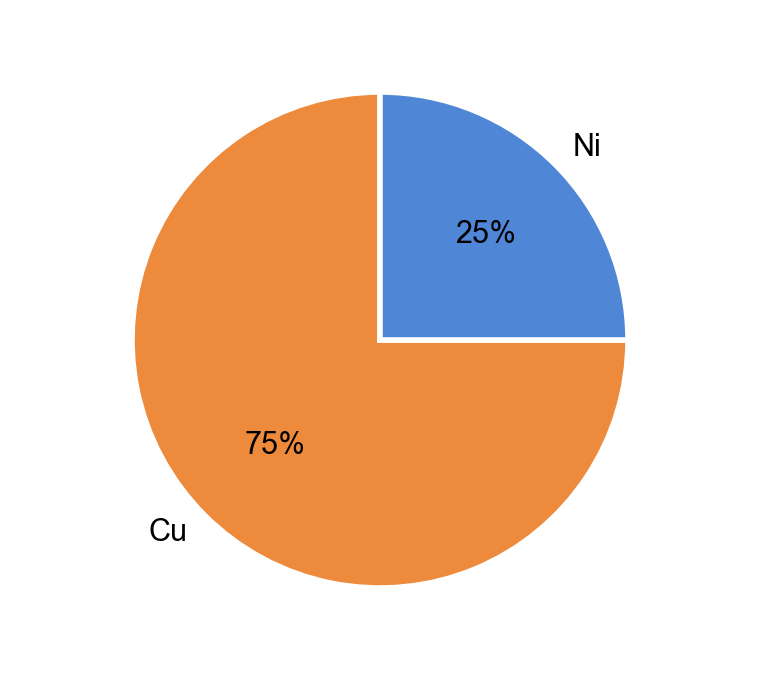
\includegraphics[width=0.86\linewidth]{rasmlar/gen/pi_v08_0.png}\end{center}
200 g qotishmadagi Ni \textbf{massasini (g) toping.}

\noindent A)~\textsl{150} \hfill B)~\textsl{100} \hfill C)~\textsl{5000} \hfill D)~\textsl{50}\par
\qsep
\noindent\qn{6.} CO va N\textsubscript{2} aralashmasi tarkibida N\textsubscript{2} ning mol miqdori CO ning mol miqdorining 4/5 qismiga teng. Aralashmaning hajmi 20,16 l (n.sh.). Aralashmaning vodorodga nisbatan \textbf{zichligini aniqlang.}

\noindent A)~\textsl{28} \hfill B)~\textsl{7} \hfill C)~\textsl{14} \hfill D)~\textsl{21}\par
\qsep
\noindent\qn{7.} pH = 2 bo`lgan HCl eritmasidan 99 ml va pH = 12 bo`lgan NaOH eritmasidan 101 ml aralashtirildi. Hosil bo`lgan eritmaning pH \textbf{ini aniqlang.}

\noindent A)~\textsl{11} \hfill B)~\textsl{10} \hfill C)~\textsl{9} \hfill D)~\textsl{7}\par
\qsep
\noindent\qn{8.} 10\% li va 25\% li tuz eritmalari massalar nisbati 1 : 1 bo`lgan holda aralashtirildi. Hosil bo`lgan eritmaning massa \textbf{ulushini (\%) hisoblang.}

\noindent A)~\textsl{14} \hfill B)~\textsl{21} \hfill C)~\textsl{17,5} \hfill D)~\textsl{35}\par
\qsep
\noindent\qn{9.} Quyidagi jadvalda NaOH tuzining eritmalari keltirilgan:
\begin{center}
\renewcommand{\arraystretch}{1.15}
\fitbox{\begin{tabular}{|c|c|c|}\hline
\textbf{No.} & \textbf{m(eritma), g} & \textbf{$\omega$, \%} \\ \hline
I & 100 & 12 \\ \hline
II & 300 & 30 \\ \hline
\end{tabular}}
\end{center}
Eritmalar aralashtirildi. Oxirgi eritmadagi tuzning massa \textbf{ulushini (\%) toping.}

\noindent A)~\textsl{21} \hfill B)~\textsl{42} \hfill C)~\textsl{25,5} \hfill D)~\textsl{16,5}\par
\qsep
\noindent\qn{10.} 0,1 mol/l li sirka kislota eritmasining 2 l ida (dissotsilanish darajasi $\alpha$ = 0,1) suv molekulalaridan tashqari jami necha mol zarracha (molekula va ionlar) bor?

\noindent A)~\textsl{0,22} \hfill B)~\textsl{0,2} \hfill C)~\textsl{0,18} \hfill D)~\textsl{0,24}\par
\qsep
\noindent\qn{11.} PCl\textsubscript{5} $\rightleftarrows$ PCl\textsubscript{3} + Cl\textsubscript{2} reaksiyasi 1 l hajmli idishda o`tkazildi. Ma'lumotlar jadvalda berilgan:
\begin{center}
\renewcommand{\arraystretch}{1.15}
\fitbox{\begin{tabular}{|c|c|c|}\hline
\textbf{Modda} & \textbf{PCl\textsubscript{5}} & \textbf{PCl\textsubscript{3}} \\ \hline
Boshlang`ich, mol & 6 & 0 \\ \hline
Muvozanatda, mol & --- & 1 \\ \hline
\end{tabular}}
\end{center}
Muvozanat \textbf{konstantasini (K) hisoblang.}

\noindent A)~\textsl{0,2} \hfill B)~\textsl{0,4} \hfill C)~\textsl{0,1} \hfill D)~\textsl{5}\par
\qsep
\noindent\qn{12.} Quyidagi jadvalda NH\textsubscript{4}NO\textsubscript{3} tuzining eritmalari keltirilgan:
\begin{center}
\renewcommand{\arraystretch}{1.15}
\fitbox{\begin{tabular}{|c|c|c|}\hline
\textbf{No.} & \textbf{m(eritma), g} & \textbf{$\omega$, \%} \\ \hline
I & 50 & 20 \\ \hline
II & 150 & 40 \\ \hline
\end{tabular}}
\end{center}
Eritmalar aralashtirildi. Oxirgi eritmadagi tuzning massa \textbf{ulushini (\%) toping.}

\noindent A)~\textsl{30} \hfill B)~\textsl{60} \hfill C)~\textsl{35} \hfill D)~\textsl{25}\par
\qsep
\noindent\qn{13.} 2SO\textsubscript{2} + O\textsubscript{2} $\rightleftarrows$ 2SO\textsubscript{3} reaksiyada muvozanat qaror topganda [SO\textsubscript{2}] = 0,5, [O\textsubscript{2}] = 3, [SO\textsubscript{3}] = 1 mol/l bo`ldi. O\textsubscript{2} ning boshlang`ich \textbf{konsentratsiyasini (mol/l) aniqlang.}

\noindent A)~\textsl{3} \hfill B)~\textsl{3,5} \hfill C)~\textsl{4} \hfill D)~\textsl{7}\par
\qsep
\noindent\qn{14.} Quyidagi jarayonlar qanday kuzatuvlar bilan boradi? To`g`ri ta'riflangan \textbf{jarayonlarni belgilang.} 1) FeCl\textsubscript{3} eritmasiga avval NaOH, so`ng mo`l HCl eritmasi qo`shilganda: qo`ng`ir-qizil cho`kma tushadi, keyin cho`kma erib, sariq eritma hosil bo`ladi; 2) NaOH eritmasiga CuSO\textsubscript{4} eritmasi tomchilab qo`shilganda (ishqor mo`l): ko`k cho`kma tushadi, keyin cho`kma erib to`q ko`k eritma hosil bo`ladi; 3) Na\textsubscript{2}CO\textsubscript{3} eritmasiga HCl eritmasi tomchilab (kislota yetishmaganda) qo`shilganda: gaz ajralmaydi (NaHCO\textsubscript{3} hosil bo`ladi), keyin kislota ko`paytirilsa ham gaz ajralmaydi; 4) CuSO\textsubscript{4} eritmasiga avval NaOH, so`ng mo`l ammiak eritmasi qo`shilganda: ko`k cho`kma tushadi, keyin cho`kma erib, to`q ko`k eritma hosil bo`ladi

\noindent A)~\textsl{1, 3, 4} \hfill B)~\textsl{4} \hfill C)~\textsl{3, 4} \hfill D)~\textsl{1, 4}\par
\qsep
\noindent\qn{15.} D-metallar va ularning birikmalari haqida qaysi fikrlar to`g`ri? 1) Temir sovuq konsentrlangan HNO\textsubscript{3} da passivlanadi; 2) Rux eritmada Fe\textsuperscript{2+} ni siqib chiqara olmaydi; 3) Cu(OH)\textsubscript{2} qizdirilganda CuO ga parchalanadi; 4) Mis suyultirilgan HCl bilan reaksiyaga kirishadi

\noindent A)~\textsl{1, 3} \hfill B)~\textsl{3} \hfill C)~\textsl{2, 4} \hfill D)~\textsl{1, 2}\par
\qsep
\noindent\qn{16.} Quyidagi oksidlardan qaysilari amfoter oksidlar? 1) SO\textsubscript{3}; 2) Cr\textsubscript{2}O\textsubscript{3}; 3) MgO; 4) CO

\noindent A)~\textsl{1, 3} \hfill B)~\textsl{2} \hfill C)~\textsl{4} \hfill D)~\textsl{3, 4}\par
\qsep
\noindent\qn{17.} PCl\textsubscript{5} $\rightleftarrows$ PCl\textsubscript{3} + Cl\textsubscript{2} reaksiyasi doimiy harorat va bosimda olib borildi; boshlang`ich modda qisman o`zgargach gazlar hajmi 3/2 marta ortdi. Boshlang`ich modda necha foizi \textbf{o`zgarganini aniqlang.}

\noindent A)~\textsl{50} \hfill B)~\textsl{25} \hfill C)~\textsl{60} \hfill D)~\textsl{100}\par
\qsep
\noindent\qn{18.} Cu $\to$ ? $\to$ ? $\to$ ? o`zgarishlar zanjirida (reagentlar: O\textsubscript{2}, H\textsubscript{2}SO\textsubscript{4}, NaOH) 1-bosqichda hosil bo`ladigan modda \textbf{formulasini toping.}

\noindent A)~\textsl{H\textsubscript{3}PO\textsubscript{4}} \hfill B)~\textsl{NaOH} \hfill C)~\textsl{CuO} \hfill D)~\textsl{Ca(OH)\textsubscript{2}}\par
\qsep
\noindent\qn{19.} 0,2 mol KClO\textsubscript{3} qizdirilganda (unum 100\%) kislorod ajraldi. Shu kislorodda oltingugurt to`liq yondirildi (S ortiqcha), hosil bo`lgan gaz 0,45 mol NaOH eritmasiga yuttirildi. Barcha reaksiyalar 1 atm bosimda olib borildi. Hosil bo`lgan tuzlar umumiy \textbf{massasini (g) toping.}

\noindent A)~\textsl{37,8} \hfill B)~\textsl{31,2} \hfill C)~\textsl{69} \hfill D)~\textsl{34,5}\par
\qsep
\noindent\qn{20.} Arenlar, neft va tabiiy gaz haqida qaysi fikrlar to`g`ri? 1) Benzolda 6 ta sp\textsuperscript{2} gibridlangan uglerod bor; 2) Naftalin -- bir halqali aren; 3) Toluol KMnO\textsubscript{4} bilan benzoy kislotagacha oksidlanadi; 4) Tabiiy gazning asosiy qismi propan

\noindent A)~\textsl{2, 4} \hfill B)~\textsl{1, 4} \hfill C)~\textsl{1, 3, 4} \hfill D)~\textsl{1, 3}\par
\qsep
\noindent\qn{21.} Murakkab efirlar va yog`lar haqida qaysi fikrlar to`g`ri? 1) Efirlanish reaksiyasi qaytmas; 2) Dietil efir spirtdan yuqori haroratda qaynaydi; 3) Etilatsetat efir hidli suyuqlik; 4) Suyuq yog`lar to`yinmagan kislotalardan hosil bo`lgan

\noindent A)~\textsl{2, 4} \hfill B)~\textsl{2} \hfill C)~\textsl{1, 3} \hfill D)~\textsl{3, 4}\par
\qsep
\noindent\qn{22.} Quyidagi birikmalardan qaysi biri fenol sinfiga kiradi?

\noindent A)~\textsl{CH\textsubscript{3}NO\textsubscript{2}} \hfill B)~\textsl{C\textsubscript{6}H\textsubscript{5}OH} \hfill C)~\textsl{C\textsubscript{2}H\textsubscript{5}NH\textsubscript{2}} \hfill D)~\textsl{CH\textsubscript{3}COCH\textsubscript{3}}\par
\qsep
\noindent\qn{23.} Formaldegid va propanal aralashmasi (14,6 g) mo`l ammiakli kumush oksid eritmasi bilan qizdirilganda 86,4 g kumush ajraldi. Reagent (ammiakli kumush oksid) eritmasining massa ulushi 36\% va zichligi 1,4 g/ml; u mo`l miqdorda olingan. Aralashmadagi formaldegidning \textbf{massasini (g) aniqlang.}

\noindent A)~\textsl{11,6} \hfill B)~\textsl{6} \hfill C)~\textsl{3} \hfill D)~\textsl{7,3}\par
\qsep
\noindent\qn{24.} Rasmda organik birikmaning tuzilish formulasi keltirilgan.
\begin{center}
\includegraphics[width=0.86\linewidth]{rasmlar/gen/fg_475166.png}\end{center}
Molekuladagi uglerod atomlari \textbf{sonini aniqlang.}

\noindent A)~\textsl{6} \hfill B)~\textsl{5} \hfill C)~\textsl{4} \hfill D)~\textsl{7}\par
\qsep
\noindent\qn{25.} 39 g C\textsubscript{6}H\textsubscript{6} dan quyidagi sxema bo`yicha 21,22 g polistirol olindi: C\textsubscript{6}H\textsubscript{6} $\to$ C\textsubscript{6}H\textsubscript{5}--C\textsubscript{2}H\textsubscript{5} $\to$ C\textsubscript{6}H\textsubscript{5}--CH=CH\textsubscript{2} $\to$ (--CH\textsubscript{2}--CH(C\textsubscript{6}H\textsubscript{5})--)n. Dastlabki 2 bosqichning unumi ketma-ket 60\%, 80\% ga teng. Barcha reaksiyalar 1 atm bosimda olib borildi. Oxirgi bosqichning \textbf{unumini (\%) aniqlang.}

\noindent A)~\textsl{85} \hfill B)~\textsl{42} \hfill C)~\textsl{15} \hfill D)~\textsl{68}\par
\qsep
\noindent\qn{26.} C\textsubscript{2}H\textsubscript{4} va C\textsubscript{4}H\textsubscript{8} aralashmasi tarkibida C\textsubscript{2}H\textsubscript{4} ning massasi aralashma massasining 1/2 qismini tashkil etadi. Aralashmaning massasi 22,4 g. Aralashmadagi C\textsubscript{2}H\textsubscript{4} ning \textbf{massasini (g) toping.}

\noindent A)~\textsl{22,4} \hfill B)~\textsl{5,6} \hfill C)~\textsl{16,8} \hfill D)~\textsl{11,2}\par
\qsep
\noindent\qn{27.} 64 g texnik CaC\textsubscript{2} (tarkibida 75\% sof modda) dan quyidagi sxema bo`yicha 10,71 g anilin olindi: CaC\textsubscript{2} $\to$ C\textsubscript{2}H\textsubscript{2} $\to$ C\textsubscript{6}H\textsubscript{6} $\to$ C\textsubscript{6}H\textsubscript{5}NO\textsubscript{2} $\to$ C\textsubscript{6}H\textsubscript{5}NH\textsubscript{2}. Dastlabki 3 bosqichning unumi ketma-ket 80\%, 80\%, 80\% ga teng. Barcha reaksiyalar 2 atm bosimda olib borildi. Oxirgi bosqichning \textbf{unumini (\%) aniqlang.}

\noindent A)~\textsl{90} \hfill B)~\textsl{45} \hfill C)~\textsl{10} \hfill D)~\textsl{72}\par
\qsep
\noindent\qn{28.} Chumoli va propion kislota aralashmasi mo`l NaHCO\textsubscript{3} eritmasi bilan ta'sirlashganda 11,2 l (n.sh.) gaz ajraldi. Shu miqdordagi aralashma ammiakli kumush oksid bilan qizdirilganda 64,8 g kumush hosil bo`ldi. Qizdirish 20 daqiqa davom etdi. Aralashmadagi propion kislotaning \textbf{massasini (g) toping.}

\noindent A)~\textsl{13,8} \hfill B)~\textsl{29,6} \hfill C)~\textsl{14,8} \hfill D)~\textsl{7,4}\par
\qsep
\noindent\qn{29.} 180 g glukoza spirtli bijg`ishga uchradi (unum 90\%). Hosil bo`lgan etanolning yarmi sirka kislotagacha oksidlandi (unum 60\%), qolgan etanol bilan sirka kislota esterlandi (unum 50\%). Barcha reaksiyalar 1 atm bosimda olib borildi. Hosil bo`lgan murakkab efir \textbf{massasini (g) hisoblang.}

\noindent A)~\textsl{47,52} \hfill B)~\textsl{11,88} \hfill C)~\textsl{23,76} \hfill D)~\textsl{35,64}\par
\qsep
\noindent\qn{30.} Quyidagi aralashmalarni ajratish usullarini mos qatorda \textbf{ko`rsating.} Aralashmalar: 1) temir va mis kukunlari; 2) etanol va suv; 3) osh tuzi va qum. Usullar: a) suvda eritish, filtrlash, bug`latish; b) ajratgich voronka yordamida; c) magnit yordamida; d) fraksiyalab haydash.

\noindent\begin{tabular}{@{}p{0.47\linewidth}@{}p{0.47\linewidth}@{}}
A)~\textsl{1-c, 2-d, 3-a} & B)~\textsl{1-b, 2-c, 3-a} \\
C)~\textsl{1-a, 2-d, 3-b} & D)~\textsl{1-a, 2-b, 3-c} \\
\end{tabular}\par
\qsep
\noindent\qn{31.} Rasmdagi asbobda NaCl ga konsentrlangan H\textsubscript{2}SO\textsubscript{4} ta'sir ettirilmoqda. Sulfat kislota bu yerda qanday vazifani bajaradi?
\begin{center}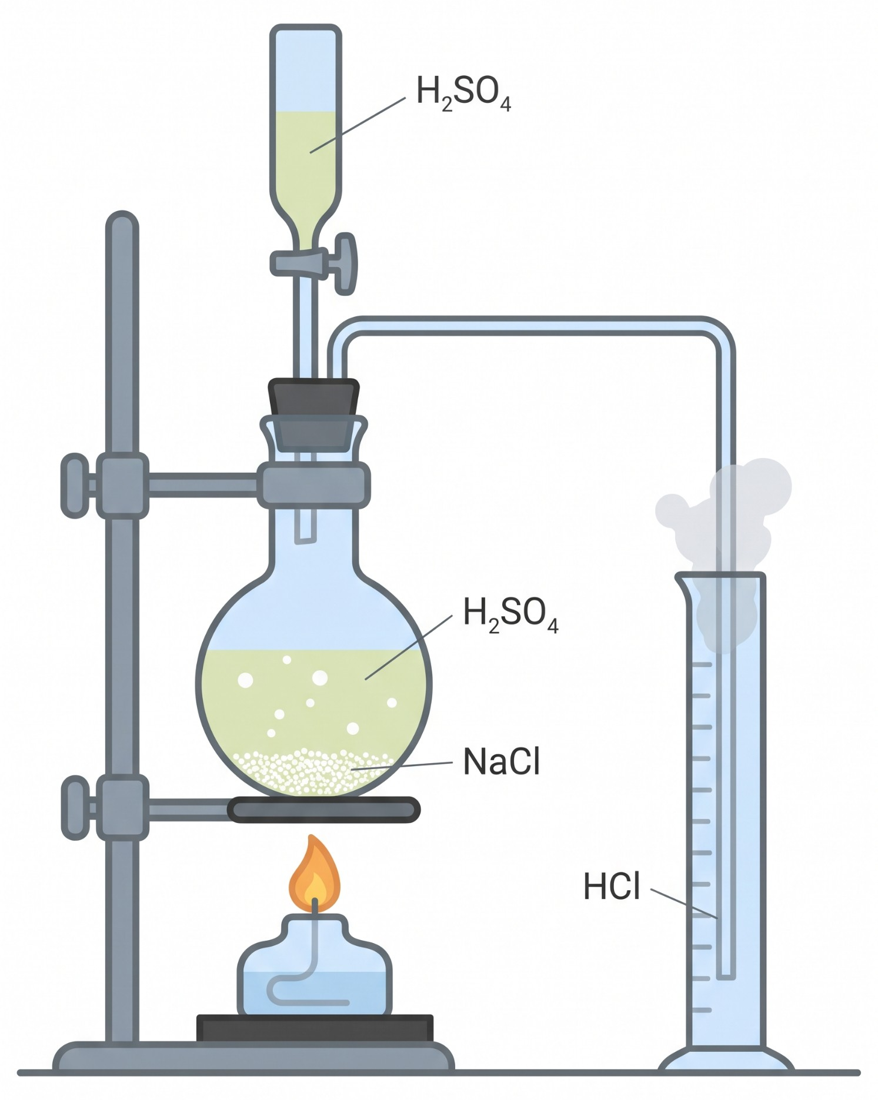
\includegraphics[width=0.86\linewidth]{rasmlar/darslik/d_hcl_lab.png}\end{center}
\noindent A)~\textsl{tuzni oksidlaydi}\par
\noindent B)~\textsl{uchuvchan bo`lmagan kuchli kislota sifatida HCl ni siqib chiqaradi}\par
\noindent C)~\textsl{reaksiyada ishtirok etmaydi}\par
\noindent D)~\textsl{faqat erituvchi vazifasini bajaradi}\par
\qsep
\noindent\qn{32.} Natriy nitrat va natriy sulfat eritmalarini (moddalarini) bir-biridan qaysi reagent yordamida farqlash mumkin?

\noindent\begin{tabular}{@{}p{0.47\linewidth}@{}p{0.47\linewidth}@{}}
A)~\textsl{bariy xlorid} & B)~\textsl{xlorid kislota} \\
C)~\textsl{natriy gidroksid} & D)~\textsl{lakmus   ---} \\
\end{tabular}\par
\qsep
\end{multicols}
\medskip
\noindent\setlength{\fboxsep}{0pt}\fbox{\begin{tabular}{p{0.74\linewidth}|p{0.2\linewidth}}
\parbox[t]{0.72\linewidth}{\vspace{3pt}\textbf{Topshiriqlar (33--35) va javob variant (A--F)larini o`zaro to`g`ri moslashtiring.} 2 mol ammiakning 9/10 qismi azot(II) oksidga oksidlandi, hosil bo`lgan oksidning 3/4 qismi nitrat kislotagacha qayta ishlandi. Kislota suvda eritilib, hajmi 13,5 l bo`lgan eritma tayyorlandi, so`ng eritma mo`l KOH bilan neytrallandi.
\vspace{3pt}} & \parbox[t]{0.19\linewidth}{\vspace{3pt}A~\textsl{75,6}\\[3pt]
B~\textsl{1,5}\\[3pt]
C~\textsl{1}\\[3pt]
D~\textsl{85,05}\\[3pt]
E~\textsl{37,8}\\[3pt]
F~\textsl{127,58}}\\ \hline
\parbox[t]{0.72\linewidth}{\vspace{2pt}\textbf{33. Hosil bo`lgan nitrat kislota massasini (g) hisoblang.}\vspace{2pt}} & \\ \hline
\parbox[t]{0.72\linewidth}{\vspace{2pt}\textbf{34. Kislota eritmasining pH ini aniqlang.}\vspace{2pt}} & \\ \hline
\parbox[t]{0.72\linewidth}{\vspace{2pt}\textbf{35. Neytrallash uchun sarflangan KOH massasini (g) toping.}\vspace{2pt}} & 
\end{tabular}}
\par\bigskip
\noindent\qn{36.} 5\% li va 30\% li tuz eritmalari massalar nisbati 3 : 2 bo`lgan holda aralashtirildi. Tajriba 20 daqiqa davom etdi. Hosil bo`lgan eritmaning massa \textbf{ulushini (\%) hisoblang.}
\javob\qsep
\noindent\qn{37.} N\textsubscript{2} + O\textsubscript{2} $\rightleftarrows$ 2NO sistemasida boshlang`ich moddalarning har biridan 1 mol dan 2 l hajmli idishga solindi. Muvozanat qaror topganda reagentlarning har birining 2/3 qismi sarflangan bo`ldi. Tajriba laboratoriyada, shisha idishda o`tkazildi. Muvozanat \textbf{konstantasini hisoblang.}
\javob\qsep
\noindent\qn{38.} Oksidlanish darajasi +2 bo`lgan noma'lum \textit{X} metallning xloridi 6,8 g massada mo`l AgNO\textsubscript{3} eritmasi bilan ta'sirlashganda 14,35 g cho`kma hosil bo`ldi. Reagent (AgNO\textsubscript{3}) eritmasining massa ulushi 10\% va zichligi 1,12 g/ml; u mo`l miqdorda olingan. \textit{X} metallning nisbiy atom \textbf{massasini toping.}
\javob\qsep
\noindent\qn{39.} 49,2 g nitrobenzol qaytarilib anilin olindi (unum 1/2). Hosil bo`lgan anilinning 2/5 qismi mo`l bromli suv bilan ta'sirlashtirildi. Hosil bo`lgan cho`kmaning \textbf{massasini (g) toping.}
\javob\qsep
\noindent\qn{40.} 49,2 g nitrobenzol qaytarilib anilin olindi (unum 3/4). Hosil bo`lgan anilinning 2/5 qismi mo`l bromli suv bilan ta'sirlashtirildi. Barcha reaksiyalar 1 atm bosimda olib borildi. Hosil bo`lgan cho`kmaning \textbf{massasini (g) toping.}
\javob\qsep
\par\bigskip\begin{center}\textbf{\fontsize{13}{15}\selectfont YOZMA ISH}\end{center}
\noindent\qn{41.} \textbf{Topshiriqni bajarish jarayonida barcha reaksiya tenglamalarini yozing. Miqdoriy va arifmetik hisoblashlarni (unga asos bo`lgan usul yoki formulani ko`rsatgan holda) uzviy ketma-ketlikda bajaring.}\par\smallskip
KX (\textit{X} -- galogen) tuzining 14,9 g namunasi mo`l AgNO\textsubscript{3} eritmasi bilan ta'sirlashganda hosil bo`lgan cho`kma massasi tuz massasidan 1,926 marta katta bo`ldi. Xuddi shunday massadagi KX namunasi MnO\textsubscript{2} va sulfat kislota bilan qizdirilib, ajralgan oddiy modda vodorod bilan to`liq reaksiyaga kiritildi, hosil bo`lgan gaz 100 g suvda eritildi. Qizdirish 15 daqiqa davom etdi. Olingan eritma 10\% li NaOH eritmasi bilan to`liq neytrallandi.\par
\noindent 1)\ KX ning AgNO\textsubscript{3} bilan reaksiyasi tenglamasini yozing va nisbatdan foydalanib \textit{X} galogenni aniqlang.\par
\noindent 2)\ KX ni MnO\textsubscript{2} va H\textsubscript{2}SO\textsubscript{4} bilan oksidlash reaksiyasini yozing; ajralgan oddiy moddaning massasini (g) va sarflangan MnO\textsubscript{2} massasini (g) hisoblang.\par
\noindent 3)\ Oddiy modda vodorod bilan reaksiyaga kirishganda hosil bo`lgan HX massasini (g) va uning suvdagi eritmasida massa ulushini (\%) toping.\par
\noindent 4)\ Neytrallash uchun sarflangan 10\% li NaOH eritmasining massasini (g) aniqlang.\par
\noindent 5)\ Neytrallangan eritmadagi NaX ning massa ulushini (\%) hisoblang.\par
\diqqat{Mazkur topshiriq kengaytirilgan javobni talab etib, uning yechilish usuli va shu usul asosidagi barcha hisoblash amallari javoblar varaqasida aks etishi lozim.}\qsep
\noindent\qn{42.} Organik moddalarning xossalarini bilgan holda reaksiya tenglamalarini tugallang va tenglashtiring. 3- va 5-reaksiyalarda hosil bo`lgan asosiy organik mahsulotlarni sistematik nomenklatura bo`yicha nomlang. Hosil bo`lgan organik moddalarning tuzilish formulalarini yozing.\par
\noindent 1)\ CH\textsubscript{3}--CH=CH\textsubscript{2} + HBr $\to$\par
\noindent 2)\ HCOOCH\textsubscript{3} + NaOH (t) $\to$\par
\noindent 3)\ CH\textsubscript{3}--CH\textsubscript{2}--OH (H\textsubscript{2}SO\textsubscript{4} kons., 170 \textdegree{}C) $\to$\par
\noindent 4)\ CH\textsubscript{3}--CHO + H\textsubscript{2} (Ni, t) $\to$\par
\noindent 5)\ CH\textsubscript{3}--NH\textsubscript{2} + HCl $\to$\par
\noindent 6)\ C\textsubscript{6}H\textsubscript{12}O\textsubscript{6} (bijg`ish) $\to$\par
\noindent 7)\ C\textsubscript{6}H\textsubscript{5}--CH\textsubscript{3} + Cl\textsubscript{2} (yorug`lik) $\to$\par
\diqqat{Mazkur topshiriq kengaytirilgan javobni talab etib, uning yechilish usuli va shu usul asosidagi barcha hisoblash amallari javoblar varaqasida aks etishi lozim.}\qsep
\noindent\qn{43.} \textbf{Topshiriqni bajarish jarayonida barcha reaksiya tenglamalarini yozing. Miqdoriy va arifmetik hisoblashlarni (unga asos bo`lgan usul yoki formulani ko`rsatgan holda) uzviy ketma-ketlikda bajaring.}\par\smallskip
NH\textsubscript{4}Cl va (NH\textsubscript{4})\textsubscript{2}SO\textsubscript{4} dan iborat 34,6 g aralashmaning bir porsiyasi mo`l NaOH eritmasi bilan qizdirilganda 13,44 l (n.sh.) gaz ajraldi. Xuddi shunday massali ikkinchi porsiya suvda eritilib, mo`l BaCl\textsubscript{2} eritmasi bilan ta'sirlashtirildi. Birinchi porsiyadan ajralgan gaz 0,5 mol H\textsubscript{3}PO\textsubscript{4} saqlagan eritmaga to`liq yuttirildi (NH\textsubscript{4}H\textsubscript{2}PO\textsubscript{4} va (NH\textsubscript{4})\textsubscript{2}HPO\textsubscript{4} aralashmasi hosil bo`ldi). Hosil bo`lgan fosfat tuzlari aralashmasi mo`l NaOH bilan qizdirilganda ajralgan gaz 300 g suvga yuttirildi va olingan eritma 10\% li HCl eritmasi bilan to`liq neytrallandi.\par
\noindent 1)\ Barcha reaksiyalarning tenglamalarini yozing va tenglashtiring. Dastlabki aralashmadagi tuzlarning massalarini (g) aniqlang.\par
\noindent 2)\ Ikkinchi porsiyada hosil bo`lgan cho`kma massasini (g) hisoblang.\par
\noindent 3)\ Fosfat kislotaga yuttirilganda hosil bo`lgan tuzlarning mol miqdorlarini toping. Fosfat tuzlari aralashmasi NaOH bilan qizdirilganda ajralgan gazning hajmini (l, n.sh.) toping.\par
\noindent 4)\ Hosil bo`lgan fosfat tuzlari aralashmasining massasini (g) va undagi azot massa ulushini (\%) aniqlang. Gaz 300 g suvga yuttirilganda eritmadagi moddaning massa ulushini (\%) hisoblang.\par
\noindent 5)\ Birinchi porsiyada ishlatilgan NaOH ning minimal massasini (g) hisoblang. Eritmani neytrallash uchun sarflangan 10\% li HCl eritmasining massasini (g) aniqlang.\par
\diqqat{Mazkur topshiriq kengaytirilgan javobni talab etib, uning yechilish usuli va shu usul asosidagi barcha hisoblash amallari javoblar varaqasida aks etishi lozim.}\qsep
\newpage
\noindent\textbf{\fontsize{13}{15}\selectfont 8-variant}\hfill \textbf{Javoblar kaliti}\par\smallskip\hrule\smallskip
\textit{Faqat o`qituvchi uchun.}\par\medskip
\noindent\textbf{1--32-savollar}\par\smallskip
\noindent\begin{tabular}{|c|c|c|c|c|c|c|c|c|c|c|c|c|c|c|c|}\hline
\textbf{1} & \textbf{2} & \textbf{3} & \textbf{4} & \textbf{5} & \textbf{6} & \textbf{7} & \textbf{8} & \textbf{9} & \textbf{10} & \textbf{11} & \textbf{12} & \textbf{13} & \textbf{14} & \textbf{15} & \textbf{16}\\\hline
\textsl{D} & \textsl{D} & \textsl{B} & \textsl{B} & \textsl{D} & \textsl{C} & \textsl{B} & \textsl{C} & \textsl{C} & \textsl{A} & \textsl{A} & \textsl{C} & \textsl{B} & \textsl{D} & \textsl{A} & \textsl{B}\\\hline
\textbf{17} & \textbf{18} & \textbf{19} & \textbf{20} & \textbf{21} & \textbf{22} & \textbf{23} & \textbf{24} & \textbf{25} & \textbf{26} & \textbf{27} & \textbf{28} & \textbf{29} & \textbf{30} & \textbf{31} & \textbf{32}\\\hline
\textsl{A} & \textsl{C} & \textsl{D} & \textsl{D} & \textsl{D} & \textsl{B} & \textsl{C} & \textsl{B} & \textsl{A} & \textsl{D} & \textsl{A} & \textsl{C} & \textsl{C} & \textsl{A} & \textsl{B} & \textsl{A}\\\hline
\end{tabular}\par\medskip
\noindent\textbf{33--35-savollar}\par\smallskip
\noindent\begin{tabular}{|c|c|c|}\hline \textbf{No} & \textbf{Javob} & \textbf{Qiymat}\\\hline
33 & \textsl{D} & 85,05\\\hline
34 & \textsl{C} & 1\\\hline
35 & \textsl{A} & 75,6\\\hline
\end{tabular}\par\medskip
\noindent\textbf{36--40-savollar}\par\smallskip
\noindent\begin{tabular}{|c|c|}\hline \textbf{No} & \textbf{To`g`ri javob}\\\hline
36 & 15\\\hline
37 & 16\\\hline
38 & 65\\\hline
39 & 26,4\\\hline
40 & 39,6\\\hline
\end{tabular}\par\medskip
\noindent\textbf{41--43-topshiriqlar: javoblar}\par\smallskip
\noindent\textbf{41-topshiriq.}\par
\noindent 1) Cl\par
\noindent 2) 7,1 g; 8,7 g\par
\noindent 3) 7,3 g; 6,8\%\par
\noindent 4) 80 g\par
\noindent 5) 6,25\%\par
\noindent\textbf{42-topshiriq.}\par
\noindent 1) CH\textsubscript{3}--CH=CH\textsubscript{2} + HBr $\to$ CH\textsubscript{3}--CHBr--CH\textsubscript{3} (Markovnikov qoidasi)\par
\noindent 2) HCOOCH\textsubscript{3} + NaOH $\to$ HCOONa + CH\textsubscript{3}OH\par
\noindent 3) CH\textsubscript{3}--CH\textsubscript{2}--OH $\to$ CH\textsubscript{2}=CH\textsubscript{2} + H\textsubscript{2}O --- nomi: \textbf{etilen}\par
\noindent 4) CH\textsubscript{3}--CHO + H\textsubscript{2} $\to$ CH\textsubscript{3}--CH\textsubscript{2}--OH\par
\noindent 5) CH\textsubscript{3}--NH\textsubscript{2} + HCl $\to$ [CH\textsubscript{3}--NH\textsubscript{3}]Cl --- nomi: \textbf{metilammoniy xlorid}\par
\noindent 6) C\textsubscript{6}H\textsubscript{12}O\textsubscript{6} $\to$ 2C\textsubscript{2}H\textsubscript{5}OH + 2CO\textsubscript{2}$\uparrow$\par
\noindent 7) C\textsubscript{6}H\textsubscript{5}--CH\textsubscript{3} + Cl\textsubscript{2} $\to$ C\textsubscript{6}H\textsubscript{5}--CH\textsubscript{2}Cl + HCl\par
\noindent\textbf{43-topshiriq.}\par
\noindent 1) 21,4 g; 13,2 g\par
\noindent 2) 23,3 g\par
\noindent 3) 0,4 mol; 0,1 mol; 13,44 l\par
\noindent 4) 59,2 g; 14,19\%; 3,29\%\par
\noindent 5) 24 g; 219 g\par
\par\bigskip\noindent\textbf{Mavzular taqsimoti}\par\smallskip
{\small\noindent\begin{longtable}{|c|p{7.2cm}|p{5.4cm}|c|}\hline \textbf{No} & \textbf{Mavzu} & \textbf{Tekshiriladigan ko`nikma} & \textbf{Ball}\\\hline
1 & Tirkashev I bob; 8-sinf (elektron konfiguratsiya) & Bilim va tushunish & 1\\\hline
2 & 11-sinf 1-bob (yadro reaksiyalari) & Bilim va tushunish & 1\\\hline
3 & 11-sinf 4-bob (molyal konsentratsiya) & Hisoblash va masala yechish & 1\\\hline
4 & Tirkashev I bob; 8-sinf (elektron konfiguratsiya) & Bilim va tushunish & 1\\\hline
5 & 8-sinf (massa ulushi, diagramma) & Grafik tahlili & 1\\\hline
6 & 8-9-sinf (gaz aralashmalari; Avogadro qonuni) & Hisoblash va masala yechish & 1\\\hline
7 & 9-sinf; 11-sinf (pH; neytrallanish) & Hisoblash va masala yechish & 1\\\hline
8 & 8-sinf (eritmalarni aralashtirish) & Hisoblash va masala yechish & 1\\\hline
9 & Tirkashev III bob (eritmalar, jadval) & Jadval tahlili & 1\\\hline
10 & 9-sinf (elektrolitik dissotsilanish) & Hisoblash va masala yechish & 1\\\hline
11 & Tirkashev VI bob (muvozanat, jadval) & Jadval tahlili & 1\\\hline
12 & Tirkashev III bob (eritmalar, jadval) & Jadval tahlili & 1\\\hline
13 & Tirkashev VI bob & Hisoblash va masala yechish & 1\\\hline
14 & 9-sinf; 11-sinf (amfoter birikmalar, kompleks hosil bo`lishi) & Bilim va tushunish & 1\\\hline
15 & 9-sinf; Tashev (Fe, Cu, Zn, Cr) & Bilim va tushunish & 1\\\hline
16 & 8-sinf; 9-sinf; Tashev (oksidlar sinflari) & Bilim va tushunish & 1\\\hline
17 & 9-11-sinf (gaz hajmi o`zgarishi; parchalanish darajasi) & Hisoblash va masala yechish & 1\\\hline
18 & 8-sinf; 9-sinf (genetik bog`lanish) & Bilim va tushunish & 1\\\hline
19 & 9-sinf (kislorod olinishi, oltingugurt oksidi + ishqor) & Hisoblash va masala yechish & 1\\\hline
20 & 10-sinf (mavzuga oid paragraflar); Abdusamatov & Bilim va tushunish & 1\\\hline
21 & 10-sinf (mavzuga oid paragraflar); Abdusamatov & Bilim va tushunish & 1\\\hline
22 & 10-sinf (organik birikmalar sinflari) & Bilim va tushunish & 1\\\hline
23 & 10-sinf (aldegidlarning kumush ko`zgu reaksiyasi) & Hisoblash va masala yechish & 1\\\hline
24 & 10-sinf (organik birikmalar) & Rasm bo`yicha tahlil & 1\\\hline
25 & 10-sinf (arenlar, polimerlar) & Hisoblash va masala yechish & 1\\\hline
26 & 10-sinf (alkenlarning brom bilan birikishi) & Hisoblash va masala yechish & 1\\\hline
27 & 10-sinf (karbiddan atsetilen, benzol, anilin) & Hisoblash va masala yechish & 1\\\hline
28 & 10-sinf (karbon kislotalar; chumoli kislotaning o`ziga xosligi) & Hisoblash va masala yechish & 1\\\hline
29 & 10-sinf (uglevodlar, spirtlar, kislotalar, efirlar) & Hisoblash va masala yechish & 1\\\hline
30 & 7-sinf (aralashmalarni ajratish); kimyoviy tahlil & Bilim va tushunish & 1\\\hline
31 & 8-sinf (17-rasm) & Rasm bo`yicha tahlil & 1\\\hline
32 & 9-sinf; 10-sinf (sifat reaksiyalari; moddalarni farqlash) & Bilim va tushunish & 1\\\hline
33--35 & Aralash masala (moslashtirish) & Ko`p bosqichli hisob & 3\\\hline
36--40 & Qisqa javobli masalalar & Hisoblash & 5\\\hline
41--43 & Yozma ish & Usul va hisob (M, A) & 75\\\hline
\end{longtable}}
\end{document}
